\PassOptionsToPackage{unicode=true}{hyperref} % options for packages loaded elsewhere
\PassOptionsToPackage{hyphens}{url}
%
\documentclass[]{article}
\usepackage{lmodern}
\usepackage{amssymb,amsmath}
\usepackage{ifxetex,ifluatex}
\usepackage{fixltx2e} % provides \textsubscript
\ifnum 0\ifxetex 1\fi\ifluatex 1\fi=0 % if pdftex
  \usepackage[T1]{fontenc}
  \usepackage[utf8]{inputenc}
  \usepackage{textcomp} % provides euro and other symbols
\else % if luatex or xelatex
  \usepackage{unicode-math}
  \defaultfontfeatures{Ligatures=TeX,Scale=MatchLowercase}
\fi
% use upquote if available, for straight quotes in verbatim environments
\IfFileExists{upquote.sty}{\usepackage{upquote}}{}
% use microtype if available
\IfFileExists{microtype.sty}{%
\usepackage[]{microtype}
\UseMicrotypeSet[protrusion]{basicmath} % disable protrusion for tt fonts
}{}
\IfFileExists{parskip.sty}{%
\usepackage{parskip}
}{% else
\setlength{\parindent}{0pt}
\setlength{\parskip}{6pt plus 2pt minus 1pt}
}
\usepackage{hyperref}
\hypersetup{
            pdftitle={WLR intervention analyses},
            pdfauthor={Matteo Lisi},
            pdfborder={0 0 0},
            breaklinks=true}
\urlstyle{same}  % don't use monospace font for urls
\usepackage[margin=1in]{geometry}
\usepackage{longtable,booktabs}
% Fix footnotes in tables (requires footnote package)
\IfFileExists{footnote.sty}{\usepackage{footnote}\makesavenoteenv{longtable}}{}
\usepackage{graphicx,grffile}
\makeatletter
\def\maxwidth{\ifdim\Gin@nat@width>\linewidth\linewidth\else\Gin@nat@width\fi}
\def\maxheight{\ifdim\Gin@nat@height>\textheight\textheight\else\Gin@nat@height\fi}
\makeatother
% Scale images if necessary, so that they will not overflow the page
% margins by default, and it is still possible to overwrite the defaults
% using explicit options in \includegraphics[width, height, ...]{}
\setkeys{Gin}{width=\maxwidth,height=\maxheight,keepaspectratio}
\setlength{\emergencystretch}{3em}  % prevent overfull lines
\providecommand{\tightlist}{%
  \setlength{\itemsep}{0pt}\setlength{\parskip}{0pt}}
\setcounter{secnumdepth}{5}
% Redefines (sub)paragraphs to behave more like sections
\ifx\paragraph\undefined\else
\let\oldparagraph\paragraph
\renewcommand{\paragraph}[1]{\oldparagraph{#1}\mbox{}}
\fi
\ifx\subparagraph\undefined\else
\let\oldsubparagraph\subparagraph
\renewcommand{\subparagraph}[1]{\oldsubparagraph{#1}\mbox{}}
\fi

% set default figure placement to htbp
\makeatletter
\def\fps@figure{htbp}
\makeatother

\usepackage{float}

\title{WLR intervention analyses}
\author{Matteo Lisi}
\date{}

\begin{document}
\maketitle

{
\setcounter{tocdepth}{4}
\tableofcontents
}
\newpage

\hypertarget{participants}{%
\section{Participants}\label{participants}}

Participants were tested at three time points: T1 (in February before
the WLR reading program), T2 (in April, after the program), and T3
(later follow up in June).

\begin{longtable}[]{@{}llrrrr@{}}
\caption{Composition of the dataset (number of subjects per
timepoint)}\tabularnewline
\toprule
Group & Nationality & refugee status & T1 & T2 & T3\tabularnewline
\midrule
\endfirsthead
\toprule
Group & Nationality & refugee status & T1 & T2 & T3\tabularnewline
\midrule
\endhead
control & Jordanian & 0 & 20 & 20 & 9\tabularnewline
WLR & Jordanian & 0 & 25 & 22 & 16\tabularnewline
control & Syrian & 1 & 22 & 12 & 9\tabularnewline
WLR & Syrian & 1 & 26 & 15 & 12\tabularnewline
\bottomrule
\end{longtable}

\begin{longtable}[]{@{}lllrr@{}}
\caption{Mean age per group and timepoint}\tabularnewline
\toprule
Group & Nationality & Timepoint & Mean age & Std.\tabularnewline
\midrule
\endfirsthead
\toprule
Group & Nationality & Timepoint & Mean age & Std.\tabularnewline
\midrule
\endhead
control & Jordanian & T1 & 8.6 & 0.9\tabularnewline
WLR & Jordanian & T1 & 8.4 & 0.9\tabularnewline
control & Syrian & T1 & 9.9 & 1.5\tabularnewline
WLR & Syrian & T1 & 8.7 & 1.4\tabularnewline
control & Jordanian & T2 & 8.6 & 0.9\tabularnewline
WLR & Jordanian & T2 & 8.6 & 0.5\tabularnewline
control & Syrian & T2 & 10.1 & 1.2\tabularnewline
WLR & Syrian & T2 & 8.5 & 1.2\tabularnewline
control & Jordanian & T3 & 9.0 & 1.0\tabularnewline
WLR & Jordanian & T3 & 8.6 & 0.5\tabularnewline
control & Syrian & T3 & 10.2 & 1.2\tabularnewline
WLR & Syrian & T3 & 8.5 & 1.2\tabularnewline
\bottomrule
\end{longtable}

\newpage

\hypertarget{modelling}{%
\section{Modelling}\label{modelling}}

To analyse the data, we used a multilevel Bayesian generalized-linear
model (GLM). The model is fully specified by the following expressions
(the first 2 define the likelihood, the rest are the priors and
hyperpriors). Note that differnetly from a classical GLM it accounts for
the possibility of lapses, or random responses (parameter \(\lambda\)).

\begin{align*}
 p(\text{responding 'sad'}) = & \frac{\lambda}{2} + (1 - \lambda) \, \Phi \left(\varphi \right)  \\
 \, \\
\varphi =  & \,  \beta_0  + u_0 + \alpha_0 \, \text{gender} + \left(\beta_1 +  u_1 + \alpha_1 \, \text{gender}\right)\, \text{img} +\beta_2\, \text{rfg} + \beta_3 \, \text{group} \\
& + \text{T2} \, \left(\beta_4 +\beta_5 \, \text{rfg} + \beta_6 \, \text{group} + \beta_7 \, \text{group} \times \text{rfg} \right) \\
& + \text{T3} \, \left(\beta_8 +\beta_9 \, \text{rfg} + \beta_{10} \, \text{group} + \beta_{11} \, \text{group} \times \text{rfg} \right)\\
& + \text{img} \, \text{T2} \, \left(\beta_{12} +\beta_{13} \, \text{rfg} + \beta_{14} \, \text{group} + \beta_{15} \, \text{group} \times \text{rfg} \right) \\
& + \text{img} \, \text{T3} \, \left(\beta_{16} +\beta_{17} \, \text{rfg} + \beta_{18} \, \text{group} + \beta_{19} \, \text{group} \times \text{rfg} \right)\\
\, \\
\beta_{0, 2, \dots, 19} \sim & \mathcal{N}\left(0, 1 \right) \\
\beta_1 \sim & \mathcal{N}\left(2, 5 \right) \\
\lambda \sim & \text{Beta} \left(0.5, 15 \right)\\
\mathbf{u} \sim & \mathcal{N}\left(0, \Sigma \right) \\
\Sigma  = & \left(\sigma_u^2 \textit{I} \right) \, \textbf{R} \, \left( \sigma_u^2 \textit{I} \right) \\
\sigma_u  \sim & \text{HalfCauchy} \left(0, 1\right)\\
\textbf{R} \sim & \text{LKJcorr} \left( 2 \right)
\end{align*}

where `img' indicate the level of morphing (centered and rescaled to
have standard deviation of 1); `rfg', `group' are dummy variables that
indicate whether the subject was a refugee (Syrian or Jordanian) or a
member of the experimental group (WLR), respectively; and `T1' and `T2'
are also dummy variables that indicate whether the measurements was
taken at T2 or T3 (the first timepoint, T1, is the baseline). `gender'
is the gender of the actor whose face was morphed to generate the
stimuli, coded using deviation (or sum) contrasts (\(\text{gender}=1\)
for female faces, and \(\text{gender}=-1\) for male faces). \(\lambda\)
is a lapse rate parameter, which is assumed to be constant for all
subjects (since it was the experimenters, not the children, who pushed
buttons for all group and at all time points). Note that the model allow
for possible differences between groups and nationality (or refugee
status), and also for differences in changes across timepoints.

Finally, note also that although the model is formulated as generalized
linear multilevel model (GLMM), the coefficients can be directly mapped
to those of the psychometric function. To see this, consider the
following simplified example:

\begin{align*}
p \left(y_i\right) & = \Phi\left(\frac{x_i -\mu}{\sigma} \right) \\
& = \Phi ( -\frac{\mu}{\sigma} + \frac{1}{\sigma}x_i )\\
& = \Phi\left(\beta_0 + \beta_1x_i \right) \\ \\& \mu=-\frac{\beta_0}{\beta_1}, \,\,\, \sigma=\frac{1}{\beta_1}
\end{align*}

\hypertarget{happy-sad-psychophysical-task}{%
\section{Happy-sad psychophysical
task}\label{happy-sad-psychophysical-task}}

The following results concern the happy-sad bias task.

The PSE, estimates via the model, are plotted in Figure 3 as a function
of the time point and group. Error bands are 95\% Bayesian credible
intervals (specifically HPDI, highest posterior density intervals).

\begin{figure}[H]

{\centering 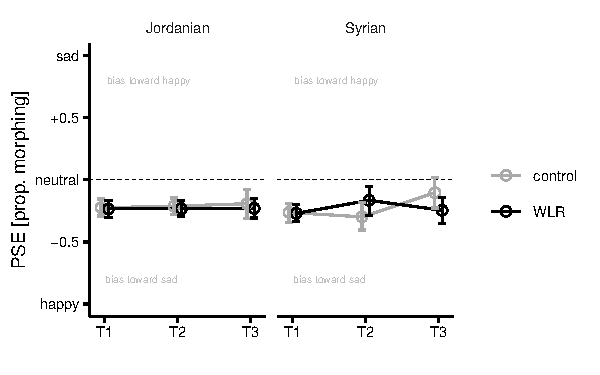
\includegraphics{WLR-analyses-report_files/figure-latex/unnamed-chunk-4-1} 

}

\caption{Group level estimate of PSE, plot by group and timepoint.}\label{fig:unnamed-chunk-4}
\end{figure}

\hypertarget{adjusting-for-differences-in-actor-identity-syrian-control-t3}{%
\subsection{Adjusting for differences in actor identity (Syrian control,
T3)}\label{adjusting-for-differences-in-actor-identity-syrian-control-t3}}

Due to a mix-up occurred while collecting data on the field, Syrian
control group at T3 was not presented with the same actors as the
others. This create a possible confound for assessing the effect of the
intervention at T3 in the Syrian group.

However, it is possible to adjust for this confound, by including in the
analysees some additiona data that we collected. Specifically, we have a
fairly large sample of Syrian children that have been tested with both
set of faces. The approach I have adopted to adjust the analysis is the
following:

\begin{enumerate}
\def\labelenumi{\arabic{enumi}.}
\item
  Estimate the difference in the parameters of the psychometric function
  using these additional dataset, which consist of the children tested
  at T1, and the new children tested at T3 (see Table 4).
\item
  Such analysis allow estimating a posterior distribution that gives the
  probability of over possible changes in the parameters due to the
  change in the identity of the stimulus.
\item
  Next, the posterior distribution is used as a prior in the full model
  (using a Gaussian approximation, see below) to constrain additional
  parameters, added to account for the effect of actor identity.
\end{enumerate}

Overall, the outcome will be identical to the previous model, except for
the estimated parameters of the Syrian control at T3, which will be
adjusted to account for the effect of actor. Importantly, using this
approach uncertainty is propagated exactly, such that the confidence
interval around the estimated parameters for the Syrian T3 group will be
larger (reflecing the added uncertainty about the true effect of actor
identity).

\begin{longtable}[]{@{}rllr@{}}
\caption{Composition of the supplementary dataset used to estimate the
effect of actor identity.}\tabularnewline
\toprule
Actor identity & Actor gender & Nationality & n. subjects\tabularnewline
\midrule
\endfirsthead
\toprule
Actor identity & Actor gender & Nationality & n. subjects\tabularnewline
\midrule
\endhead
1 & F & Syrian & 26\tabularnewline
2 & F & Syrian & 11\tabularnewline
1 & M & Syrian & 23\tabularnewline
2 & M & Syrian & 11\tabularnewline
\bottomrule
\end{longtable}

The model is a simplified version of the full model described above,
with the difference that in this case there are no parameter to code for
group effects, but only for the effect of actor gender and identity. The
simplified model is fully specified by the following expressions:

\begin{align*}
 p(\text{responding 'sad'}) = & \frac{\lambda}{2} + (1 - \lambda) \, \Phi \left(\varphi \right)  \\
 \, \\
\varphi =  & \,  \beta_0  + u_0 + \beta_2 \, \text{gender} +\beta_3\, \text{actor} + \beta_4 \, \text{gender} \times \text{actor} \\
 & +  \text{img} \, \left(\beta_1 +  u_1 + \beta_5 \, \text{gender} +\beta_6\, \text{actor} + \beta_7 \, \text{gender} \times \text{actor} \right) \\
\, \\
\beta_{0, 2, \dots, 7} \sim & \mathcal{N}\left(0, 1 \right) \\
\beta_1 \sim & \mathcal{N}\left(2, 5 \right) \\
\lambda \sim & \text{Beta} \left(0.5, 15 \right)\\
\mathbf{u} \sim & \mathcal{N}\left(0, \Sigma \right) \\
\Sigma  = & \left(\sigma_u^2 \textit{I} \right) \, \textbf{R} \, \left( \sigma_u^2 \textit{I} \right) \\
\sigma_u  \sim & \text{HalfCauchy} \left(0, 1\right)\\
\textbf{R} \sim & \text{LKJcorr} \left( 2 \right)
\end{align*}

The posterior distribution obtained for the parameters of interest
(i.e., \(\beta_3, \beta_4, \beta_6, \beta_7\)) are shown in the next
figure. The histogram represents the samples of the posterior
distribution obtained via Markov-Chain Montecarlo (MCMC) sampling. The
red curves are Gaussian functions, fit on the posterior samples, which
will be used to

\begin{figure}[H]

{\centering 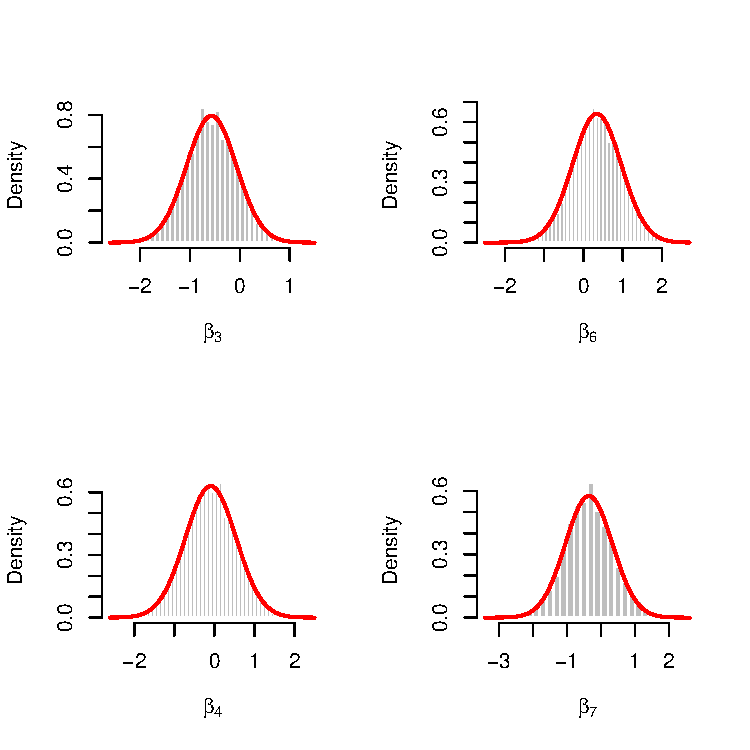
\includegraphics{WLR-analyses-report_files/figure-latex/unnamed-chunk-6-1} 

}

\caption{The grey histogram shows the posterior distributions over the effect of actor identity on bias and psychometric slopes. Red lines are the Gaussian approximation that was used the as informative prior in the main analysis.}\label{fig:unnamed-chunk-6}
\end{figure}

\begin{longtable}[]{@{}llrr@{}}
\caption{Summary statistics for posterior distributions of the effect of
actor identity.}\tabularnewline
\toprule
Parameter & name.in.updated.model & Mean & Std\tabularnewline
\midrule
\endfirsthead
\toprule
Parameter & name.in.updated.model & Mean & Std\tabularnewline
\midrule
\endhead
beta\_3 & beta\_20 & -0.569 & 0.502\tabularnewline
beta\_4 & beta\_21 & -0.092 & 0.634\tabularnewline
beta\_6 & beta\_22 & 0.341 & 0.621\tabularnewline
beta\_7 & beta\_23 & -0.356 & 0.692\tabularnewline
\bottomrule
\end{longtable}

The posterior distribution, summarized in the table, are then used as
prior in the updated model used to analyze the effect of the
intervention, which becomes

\begin{align*}
 p(\text{responding 'sad'}) = & \frac{\lambda}{2} + (1 - \lambda) \, \Phi \left(\varphi \right)  \\
 \, \\
\varphi =  & \,  \beta_0  + u_0 + \alpha_0 \, \text{gender} + \left(\beta_1 +  u_1 + \alpha_1 \, \text{gender}\right)\, \text{img} +\beta_2\, \text{rfg} + \beta_3 \, \text{group} \\
& + \text{T2} \, \left(\beta_4 +\beta_5 \, \text{rfg} + \beta_6 \, \text{group} + \beta_7 \, \text{group} \times \text{rfg} \right) \\
& + \text{T3} \, \left(\beta_8 +\beta_9 \, \text{rfg} + \beta_{10} \, \text{group} + \beta_{11} \, \text{group} \times \text{rfg} \right)\\
& + \text{img} \, \text{T2} \, \left(\beta_{12} +\beta_{13} \, \text{rfg} + \beta_{14} \, \text{group} + \beta_{15} \, \text{group} \times \text{rfg} \right) \\
& + \text{img} \, \text{T3} \, \left(\beta_{16} +\beta_{17} \, \text{rfg} + \beta_{18} \, \text{group} + \beta_{19} \, \text{group} \times \text{rfg} \right)\\
& + \beta_{20} \, \text{actor} + \beta_{21} \, \text{gender} \times \text{actor}\\
& + \text{img} \left( \beta_{22} \, \text{actor} + \beta_{23} \, \text{gender} \times \text{actor} \right)
\end{align*}

where I have added to the bottom the new part (last two lines), and
omitted the prior description for brevity. The prior description is the
same as before, with the exception that the new parameters
\(\beta_{20}, \dots, \beta_{23}\) have priors that are normal
distribution with mean and standard deviation as indicated in the table
(i.e.~they correspond to the red curves). The results of this new
analysis are represented in Figure 6. Notice that the main differences
are that while previously the Syrian control seemed to exhibit an
decrease in bias at T3, this effect can be entirely explained by the
change in stimulus. The confidence bands is increased to reflect the
increased uncertainty, however it seems safe to conclude that these
results indicate that the none of the control groups, Syrian or
Jordanian, exhibited significant changes in bias across timepoints.

\begin{figure}[H]

{\centering 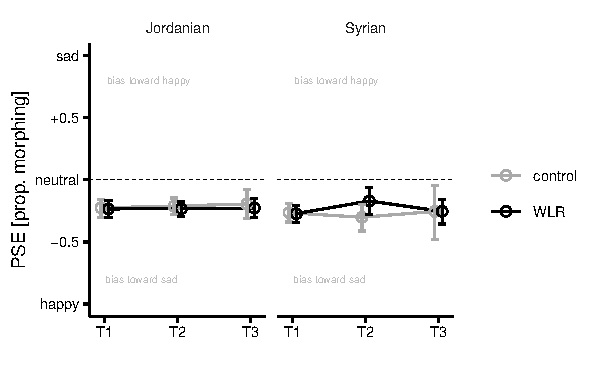
\includegraphics{WLR-analyses-report_files/figure-latex/unnamed-chunk-8-1} 

}

\caption{Group level estimate of PSE, plot by group and timepoint. Estimated using all data, and with adjustment for the bias of Syrian control at T3, due to the different stimulus (see text).}\label{fig:unnamed-chunk-8}
\end{figure}

This can be seen even more clearly in Figure 7, where the same data is
plotted as differences from T1

\begin{figure}[H]

{\centering 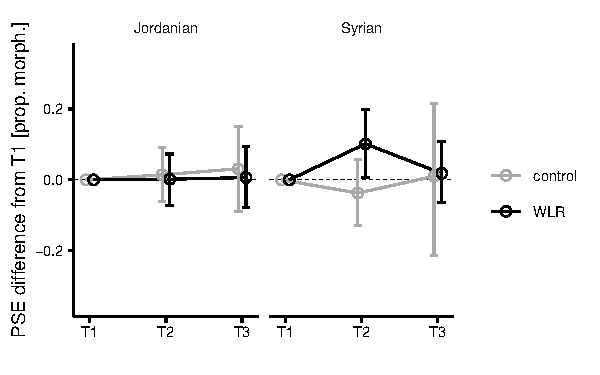
\includegraphics{WLR-analyses-report_files/figure-latex/unnamed-chunk-9-1} 

}

\caption{Group level estimate of PSE, plotted as a difference from T1.}\label{fig:unnamed-chunk-9}
\end{figure}

\begin{longtable}[]{@{}lllrrrr@{}}
\caption{Mean and 95\% credible intervals of differences from T1
(happy-sad task).}\tabularnewline
\toprule
time & ethni & group & mu & mu\_se & mu\_lb & mu\_ub\tabularnewline
\midrule
\endfirsthead
\toprule
time & ethni & group & mu & mu\_se & mu\_lb & mu\_ub\tabularnewline
\midrule
\endhead
T2 & Syrian & control & -0.037 & 0.048 & -0.130 & 0.057\tabularnewline
T2 & Syrian & WLR & 0.102 & 0.050 & 0.007 & 0.199\tabularnewline
T2 & Jordanian & control & 0.014 & 0.039 & -0.061 & 0.092\tabularnewline
T2 & Jordanian & WLR & 0.002 & 0.037 & -0.073 & 0.073\tabularnewline
T3 & Syrian & control & 0.010 & 0.111 & -0.213 & 0.216\tabularnewline
T3 & Syrian & WLR & 0.018 & 0.044 & -0.065 & 0.109\tabularnewline
T3 & Jordanian & control & 0.031 & 0.061 & -0.089 & 0.151\tabularnewline
T3 & Jordanian & WLR & 0.006 & 0.044 & -0.079 & 0.095\tabularnewline
\bottomrule
\end{longtable}

\newpage

\hypertarget{fear-anger-psychophysical-task}{%
\section{Fear-anger psychophysical
task}\label{fear-anger-psychophysical-task}}

Analyses of the fear-anger task. The analysis procedure is exactly the
same.

The only difference is that in this case I have two Jordanian control
that were tested using actor 2 at T3, therefore in the additional model
used to estimate the effect of the actor identity I have included both
Syrian and Jordanian (see table). The results indicates no effect of the
treatment, since the confidence intervals are always largely
overlapping. There is a significant change in bias at T2 but only for
the Jordanians, and for both the control and experimental group.

\begin{longtable}[]{@{}rllr@{}}
\caption{Composition of the supplementary dataset used to estimate the
effect of actor identity.}\tabularnewline
\toprule
Actor identity & Actor gender & Nationality & n. subjects\tabularnewline
\midrule
\endfirsthead
\toprule
Actor identity & Actor gender & Nationality & n. subjects\tabularnewline
\midrule
\endhead
1 & F & Jordanian & 23\tabularnewline
2 & F & Jordanian & 8\tabularnewline
1 & M & Jordanian & 23\tabularnewline
2 & M & Jordanian & 8\tabularnewline
1 & F & Syrian & 23\tabularnewline
2 & F & Syrian & 11\tabularnewline
1 & M & Syrian & 26\tabularnewline
2 & M & Syrian & 11\tabularnewline
\bottomrule
\end{longtable}

Figure 10 and 11 represent the PSE in the FA task, using the same
coventions adopted in the previous figures.

\begin{figure}[H]

{\centering 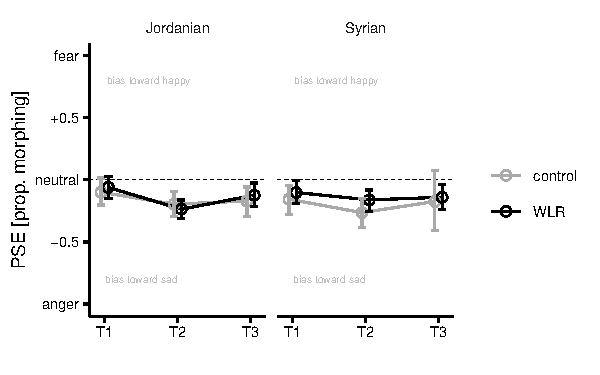
\includegraphics{WLR-analyses-report_files/figure-latex/unnamed-chunk-12-1} 

}

\caption{Group level estimate of PSE in the FA task, plot by group and timepoint. Estimated using all data, and with adjustment for the bias of Syrian control at T3, due to the different stimulus (see text).}\label{fig:unnamed-chunk-12}
\end{figure}

\begin{figure}[H]

{\centering 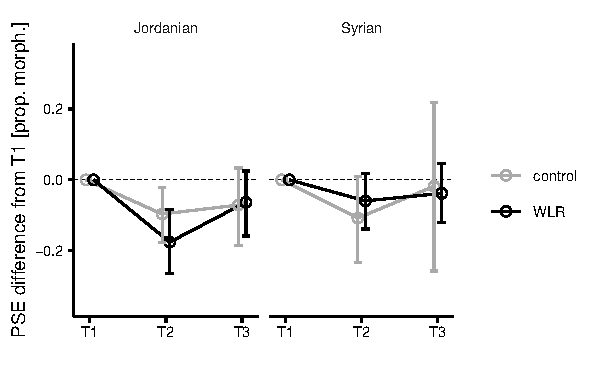
\includegraphics{WLR-analyses-report_files/figure-latex/unnamed-chunk-13-1} 

}

\caption{Group level estimate of PSE, plotted as a difference from T1.}\label{fig:unnamed-chunk-13}
\end{figure}

\begin{longtable}[]{@{}lllrrrr@{}}
\caption{Mean and 95\% credible intervals of differences from T1
(fear-anger task).}\tabularnewline
\toprule
time & ethni & group & mu & mu\_se & mu\_lb & mu\_ub\tabularnewline
\midrule
\endfirsthead
\toprule
time & ethni & group & mu & mu\_se & mu\_lb & mu\_ub\tabularnewline
\midrule
\endhead
T2 & Syrian & control & -0.108 & 0.062 & -0.234 & 0.010\tabularnewline
T2 & Syrian & WLR & -0.059 & 0.040 & -0.138 & 0.017\tabularnewline
T2 & Jordanian & control & -0.096 & 0.040 & -0.177 &
-0.021\tabularnewline
T2 & Jordanian & WLR & -0.176 & 0.047 & -0.265 & -0.083\tabularnewline
T3 & Syrian & control & -0.018 & 0.123 & -0.257 & 0.219\tabularnewline
T3 & Syrian & WLR & -0.038 & 0.042 & -0.121 & 0.046\tabularnewline
T3 & Jordanian & control & -0.071 & 0.056 & -0.186 &
0.033\tabularnewline
T3 & Jordanian & WLR & -0.063 & 0.047 & -0.158 & 0.025\tabularnewline
\bottomrule
\end{longtable}

\newpage

\hypertarget{questionnaires-analysis}{%
\section{Questionnaires analysis}\label{questionnaires-analysis}}

\hypertarget{whole-sample-comparison-at-t1}{%
\subsection{Whole-sample comparison at
T1}\label{whole-sample-comparison-at-t1}}

The different questionnaire measures obtained at T1 where compared
across groups (Syrian vs.~Jordanian) using the Mann--Whitney \emph{U}
test, with a normal approximation to compute the p-values. See table for
the results

\begin{longtable}[]{@{}lrr@{}}
\caption{Comparison of questionnaire responses at T1 (Syrian vs
Jordanian). TEC = Traumatic Events}\tabularnewline
\toprule
questionnaire & W & p\tabularnewline
\midrule
\endfirsthead
\toprule
questionnaire & W & p\tabularnewline
\midrule
\endhead
OPTIMISM\_1 & 1314.0 & 0.0904962\tabularnewline
PPL\_IN\_HOUSEHOLD & 996.5 & 0.4157287\tabularnewline
CRIES\_8 & 811.0 & 0.1240409\tabularnewline
CRIES\_INTRUSION & 831.5 & 0.0893334\tabularnewline
CRIES\_AVOIDANCE & 909.5 & 0.2126538\tabularnewline
AYMHS\_1 & 1000.5 & 0.9258415\tabularnewline
HIDS\_INSECURITY\_1 & 1153.5 & 0.2537263\tabularnewline
HIDS\_DISTRESS\_1 & 1036.0 & 0.9904620\tabularnewline
TEC & 82.0 & 0.0000000\tabularnewline
CRIES\_ADJUSTED & 615.0 & 0.0000187\tabularnewline
CRIES\_SCORE & 710.0 & 0.0002571\tabularnewline
\bottomrule
\end{longtable}

Longitudinal tests for changes in the questionnaire scores at the
different time points were done using the non-parametric marginal model
(Brunner and Puri 2001,@Brunner1999), a generalization of classical
non-parametric tests to repeated-measures, factorial designs. For each
test the statistical significance is assessed using the ANOVA-type
statistic (ATS). The ATS is typically preferred to more classical
\(\chi^2\) commonly used by rank-score tests as it requires less
assumptions on the covariance matrix and it has superior small sample
performances (Brunner and Puri 2001). Moreover, for the main effects and
interactions involving only the between subjects effects, I report the
modified ANOVA-type statistic with Box approximation, which is preferred
to ATS (Brunner and Puri 2001).

Notice that the longitudinal tests are restricted to the subset of
participants for which a measure is available at all timepoints.

\newpage

\hypertarget{group-comparisn-of-tec-at-t1}{%
\subsection{Group comparisn of TEC at
T1}\label{group-comparisn-of-tec-at-t1}}

\begin{longtable}[]{@{}lrr@{}}
\caption{Mean TEC scores at T1 by group}\tabularnewline
\toprule
& Control & WLR\tabularnewline
\midrule
\endfirsthead
\toprule
& Control & WLR\tabularnewline
\midrule
\endhead
Jordanian & 0.15 & 0.20\tabularnewline
Syrian & 9.86 & 5.67\tabularnewline
\bottomrule
\end{longtable}

\begin{longtable}[]{@{}lrr@{}}
\caption{Std TEC scores at T1 by group}\tabularnewline
\toprule
& Control & WLR\tabularnewline
\midrule
\endfirsthead
\toprule
& Control & WLR\tabularnewline
\midrule
\endhead
Jordanian & 0.37 & 0.50\tabularnewline
Syrian & 2.01 & 3.61\tabularnewline
\bottomrule
\end{longtable}

\begin{longtable}[]{@{}lrrrr@{}}
\caption{Insecurity: ANOVA-Type Statistc. TEC at T1 time
point}\tabularnewline
\toprule
& Statistic & df1 & df2 & p-Value\tabularnewline
\midrule
\endfirsthead
\toprule
& Statistic & df1 & df2 & p-Value\tabularnewline
\midrule
\endhead
wlr\_group & 16.51701 & 1 & 76.03479 & 0.000116\tabularnewline
nationality & 330.04831 & 1 & 76.03479 & 0.000000\tabularnewline
wlr\_group:nationality & 17.93002 & 1 & 76.03479 &
0.000064\tabularnewline
\bottomrule
\end{longtable}

\newpage

\hypertarget{longitudinal-analysis-3-time-points}{%
\subsection{Longitudinal analysis (3 time
points)}\label{longitudinal-analysis-3-time-points}}

The following plots contain data from all participants (regardless of
whether they showed up at T2 or T3).

\hypertarget{optimism}{%
\subsubsection{Optimism}\label{optimism}}

\begin{figure}[H]

{\centering 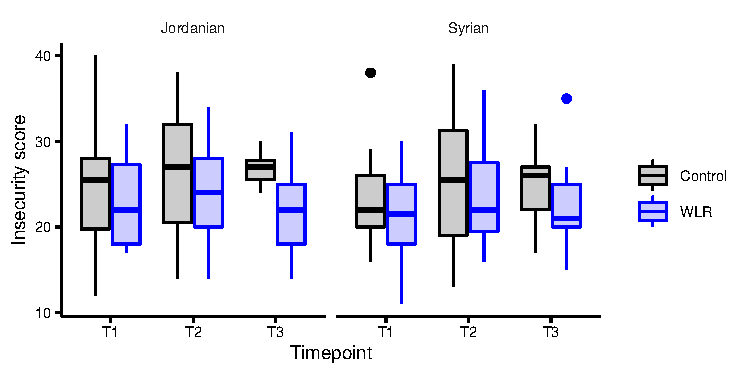
\includegraphics{WLR-analyses-report_files/figure-latex/unnamed-chunk-19-1} 

}

\caption{Optimism scores across timepoints}\label{fig:unnamed-chunk-19}
\end{figure}

\begin{longtable}[]{@{}lrrr@{}}
\caption{Optimism: ANOVA-Type Statistc (ATS).}\tabularnewline
\toprule
& Statistic & df & p-value\tabularnewline
\midrule
\endfirsthead
\toprule
& Statistic & df & p-value\tabularnewline
\midrule
\endhead
wlr\_group & 3.5923634 & 1.000000 & 0.0580456\tabularnewline
nationality & 4.9052342 & 1.000000 & 0.0267754\tabularnewline
time & 3.4456288 & 1.837244 & 0.0357247\tabularnewline
wlr\_group:nationality & 1.0709478 & 1.000000 & 0.3007315\tabularnewline
wlr\_group:time & 1.3613788 & 1.837244 & 0.2560062\tabularnewline
nationality:time & 0.8612858 & 1.837244 & 0.4144877\tabularnewline
wlr\_group:nationality:time & 1.4252773 & 1.837244 &
0.2408272\tabularnewline
\bottomrule
\end{longtable}

\begin{longtable}[]{@{}lrrrr@{}}
\caption{Optimism: Modified ANOVA-Type Statistic for the
between-subjects factors.}\tabularnewline
\toprule
& Statistic & df1 & df2 & p-value\tabularnewline
\midrule
\endfirsthead
\toprule
& Statistic & df1 & df2 & p-value\tabularnewline
\midrule
\endhead
wlr\_group & 3.592363 & 1 & 25.94952 & 0.0692370\tabularnewline
nationality & 4.905234 & 1 & 25.94952 & 0.0357630\tabularnewline
wlr\_group:nationality & 1.070948 & 1 & 25.94952 &
0.3102799\tabularnewline
\bottomrule
\end{longtable}

\newpage

\hypertarget{human-insecurity-scale-his}{%
\subsubsection{Human Insecurity Scale
(HIS)}\label{human-insecurity-scale-his}}

\begin{figure}[H]

{\centering 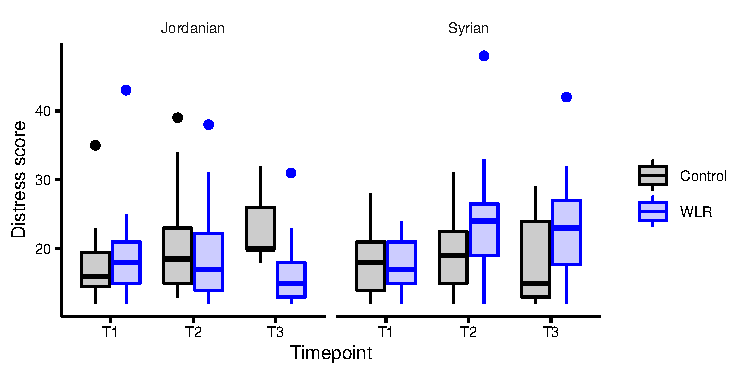
\includegraphics{WLR-analyses-report_files/figure-latex/unnamed-chunk-22-1} 

}

\caption{Insecurity scores across timepoints}\label{fig:unnamed-chunk-22}
\end{figure}

\begin{longtable}[]{@{}lrrr@{}}
\caption{Insecurity: ANOVA-Type Statistc (ATS).}\tabularnewline
\toprule
& Statistic & df & p-value\tabularnewline
\midrule
\endfirsthead
\toprule
& Statistic & df & p-value\tabularnewline
\midrule
\endhead
wlr\_group & 2.2265276 & 1.000000 & 0.1356584\tabularnewline
nationality & 2.9460533 & 1.000000 & 0.0860876\tabularnewline
time & 1.8402814 & 1.589945 & 0.1671087\tabularnewline
wlr\_group:nationality & 0.0001575 & 1.000000 & 0.9899877\tabularnewline
wlr\_group:time & 1.3898812 & 1.589945 & 0.2482679\tabularnewline
nationality:time & 0.3437137 & 1.589945 & 0.6592568\tabularnewline
wlr\_group:nationality:time & 1.0947785 & 1.589945 &
0.3234342\tabularnewline
\bottomrule
\end{longtable}

\begin{longtable}[]{@{}lrrrr@{}}
\caption{Insecurity: Modified ANOVA-Type Statistic for the
between-subjects factors.}\tabularnewline
\toprule
& Statistic & df1 & df2 & p-value\tabularnewline
\midrule
\endfirsthead
\toprule
& Statistic & df1 & df2 & p-value\tabularnewline
\midrule
\endhead
wlr\_group & 2.2265276 & 1 & 11.15105 & 0.1633990\tabularnewline
nationality & 2.9460533 & 1 & 11.15105 & 0.1137017\tabularnewline
wlr\_group:nationality & 0.0001575 & 1 & 11.15105 &
0.9902094\tabularnewline
\bottomrule
\end{longtable}

\newpage

\hypertarget{human-distress-scale-hds}{%
\subsubsection{Human Distress Scale
(HDS)}\label{human-distress-scale-hds}}

\begin{figure}[H]

{\centering 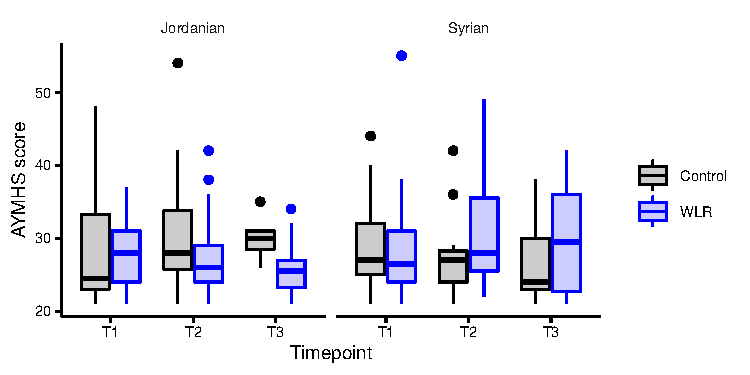
\includegraphics{WLR-analyses-report_files/figure-latex/unnamed-chunk-25-1} 

}

\caption{Distress scores across timepoints}\label{fig:unnamed-chunk-25}
\end{figure}

\begin{longtable}[]{@{}lrrr@{}}
\caption{Distress: ANOVA-Type Statistc (ATS).}\tabularnewline
\toprule
& Statistic & df & p-value\tabularnewline
\midrule
\endfirsthead
\toprule
& Statistic & df & p-value\tabularnewline
\midrule
\endhead
wlr\_group & 0.1665382 & 1.000000 & 0.6832069\tabularnewline
nationality & 0.0241826 & 1.000000 & 0.8764211\tabularnewline
time & 4.1466123 & 1.593206 & 0.0235174\tabularnewline
wlr\_group:nationality & 3.9598536 & 1.000000 & 0.0465978\tabularnewline
wlr\_group:time & 0.9117982 & 1.593206 & 0.3823730\tabularnewline
nationality:time & 0.2685269 & 1.593206 & 0.7132980\tabularnewline
wlr\_group:nationality:time & 6.1912807 & 1.593206 &
0.0043112\tabularnewline
\bottomrule
\end{longtable}

\begin{longtable}[]{@{}lrrrr@{}}
\caption{Distress: Modified ANOVA-Type Statistic for the
between-subjects factors.}\tabularnewline
\toprule
& Statistic & df1 & df2 & p-value\tabularnewline
\midrule
\endfirsthead
\toprule
& Statistic & df1 & df2 & p-value\tabularnewline
\midrule
\endhead
wlr\_group & 0.1665382 & 1 & 29.29467 & 0.6861744\tabularnewline
nationality & 0.0241826 & 1 & 29.29467 & 0.8774877\tabularnewline
wlr\_group:nationality & 3.9598536 & 1 & 29.29467 &
0.0560033\tabularnewline
\bottomrule
\end{longtable}

\newpage

\hypertarget{arab-youth-mental-health-scale-aymhs}{%
\subsubsection{Arab Youth Mental Health Scale
(AYMHS)}\label{arab-youth-mental-health-scale-aymhs}}

\begin{figure}[H]

{\centering 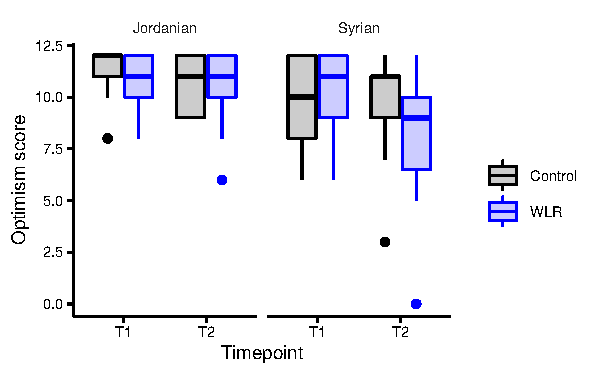
\includegraphics{WLR-analyses-report_files/figure-latex/unnamed-chunk-28-1} 

}

\caption{Mental health (AYMHS) scores across timepoints}\label{fig:unnamed-chunk-28}
\end{figure}

\begin{longtable}[]{@{}lrrr@{}}
\caption{Mental health (AYMHS): ANOVA-Type Statistc
(ATS).}\tabularnewline
\toprule
& Statistic & df & p-value\tabularnewline
\midrule
\endfirsthead
\toprule
& Statistic & df & p-value\tabularnewline
\midrule
\endhead
wlr\_group & 0.0019947 & 1.00000 & 0.9643769\tabularnewline
nationality & 0.6386774 & 1.00000 & 0.4241901\tabularnewline
time & 6.2171464 & 1.58446 & 0.0042890\tabularnewline
wlr\_group:nationality & 1.7724457 & 1.00000 & 0.1830797\tabularnewline
wlr\_group:time & 0.7615615 & 1.58446 & 0.4389209\tabularnewline
nationality:time & 1.4786086 & 1.58446 & 0.2294960\tabularnewline
wlr\_group:nationality:time & 4.0916958 & 1.58446 &
0.0248288\tabularnewline
\bottomrule
\end{longtable}

\begin{longtable}[]{@{}lrrrr@{}}
\caption{Mental health (AYMHS): Modified ANOVA-Type Statistic for the
between-subjects factors.}\tabularnewline
\toprule
& Statistic & df1 & df2 & p-value\tabularnewline
\midrule
\endfirsthead
\toprule
& Statistic & df1 & df2 & p-value\tabularnewline
\midrule
\endhead
wlr\_group & 0.0019947 & 1 & 28.12391 & 0.9646925\tabularnewline
nationality & 0.6386774 & 1 & 28.12391 & 0.4308882\tabularnewline
wlr\_group:nationality & 1.7724457 & 1 & 28.12391 &
0.1937713\tabularnewline
\bottomrule
\end{longtable}

\newpage

\hypertarget{longitudinal-analysis-2-time-points}{%
\subsection{Longitudinal analysis (2 time
points)}\label{longitudinal-analysis-2-time-points}}

The following plots contain data from only participants that were
re-tested at T2.

\hypertarget{optimism-1}{%
\subsubsection{Optimism}\label{optimism-1}}

\begin{figure}[H]

{\centering 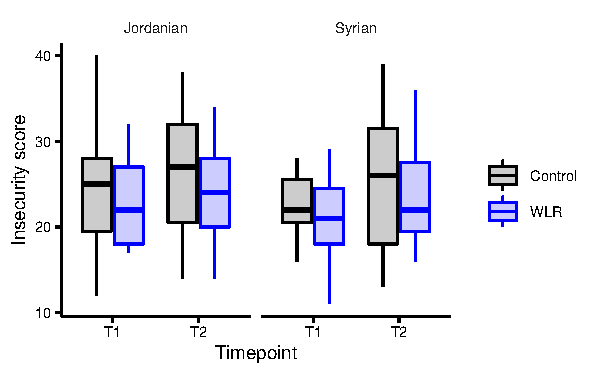
\includegraphics{WLR-analyses-report_files/figure-latex/unnamed-chunk-31-1} 

}

\caption{Optimism scores across 2 timepoints}\label{fig:unnamed-chunk-31}
\end{figure}

\begin{longtable}[]{@{}lrrr@{}}
\caption{Optimism: ANOVA-Type Statistc (ATS). 2 time points
only.}\tabularnewline
\toprule
& Statistic & df & p-value\tabularnewline
\midrule
\endfirsthead
\toprule
& Statistic & df & p-value\tabularnewline
\midrule
\endhead
wlr\_group & 2.0382184 & 1 & 0.1533892\tabularnewline
nationality & 4.7440722 & 1 & 0.0293994\tabularnewline
time & 9.1556824 & 1 & 0.0024795\tabularnewline
wlr\_group:nationality & 0.2938879 & 1 & 0.5877398\tabularnewline
wlr\_group:time & 0.1886453 & 1 & 0.6640465\tabularnewline
nationality:time & 0.0394533 & 1 & 0.8425534\tabularnewline
wlr\_group:nationality:time & 4.0472755 & 1 & 0.0442427\tabularnewline
\bottomrule
\end{longtable}

\begin{longtable}[]{@{}lrrrr@{}}
\caption{Optimism: Modified ANOVA-Type Statistic for the
between-subjects factors. 2 time points only.}\tabularnewline
\toprule
& Statistic & df1 & df2 & p-value\tabularnewline
\midrule
\endfirsthead
\toprule
& Statistic & df1 & df2 & p-value\tabularnewline
\midrule
\endhead
wlr\_group & 2.0382184 & 1 & 42.05632 & 0.1607730\tabularnewline
nationality & 4.7440722 & 1 & 42.05632 & 0.0350566\tabularnewline
wlr\_group:nationality & 0.2938879 & 1 & 42.05632 &
0.5906008\tabularnewline
\bottomrule
\end{longtable}

\newpage

\hypertarget{human-insecurity-scale-his-1}{%
\subsubsection{Human Insecurity Scale
(HIS)}\label{human-insecurity-scale-his-1}}

\begin{figure}[H]

{\centering 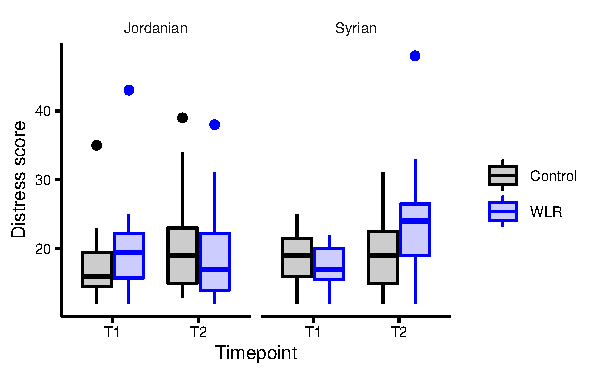
\includegraphics{WLR-analyses-report_files/figure-latex/unnamed-chunk-34-1} 

}

\caption{Insecurity scores across 2 timepoints}\label{fig:unnamed-chunk-34}
\end{figure}

\begin{longtable}[]{@{}lrrr@{}}
\caption{Insecurity: ANOVA-Type Statistc (ATS). 2 time points
only.}\tabularnewline
\toprule
& Statistic & df & p-value\tabularnewline
\midrule
\endfirsthead
\toprule
& Statistic & df & p-value\tabularnewline
\midrule
\endhead
wlr\_group & 1.2846914 & 1 & 0.2570286\tabularnewline
nationality & 0.6141009 & 1 & 0.4332479\tabularnewline
time & 3.8104314 & 1 & 0.0509343\tabularnewline
wlr\_group:nationality & 0.0012357 & 1 & 0.9719579\tabularnewline
wlr\_group:time & 0.0484404 & 1 & 0.8257997\tabularnewline
nationality:time & 0.4908202 & 1 & 0.4835617\tabularnewline
wlr\_group:nationality:time & 0.3493180 & 1 & 0.5544994\tabularnewline
\bottomrule
\end{longtable}

\begin{longtable}[]{@{}lrrrr@{}}
\caption{Insecurity: Modified ANOVA-Type Statistic for the
between-subjects factors. 2 time points only.}\tabularnewline
\toprule
& Statistic & df1 & df2 & p-value\tabularnewline
\midrule
\endfirsthead
\toprule
& Statistic & df1 & df2 & p-value\tabularnewline
\midrule
\endhead
wlr\_group & 1.2846914 & 1 & 45.37821 & 0.2629815\tabularnewline
nationality & 0.6141009 & 1 & 45.37821 & 0.4373192\tabularnewline
wlr\_group:nationality & 0.0012357 & 1 & 45.37821 &
0.9721121\tabularnewline
\bottomrule
\end{longtable}

\newpage

\hypertarget{human-distress-scale-hds-1}{%
\subsubsection{Human Distress Scale
(HDS)}\label{human-distress-scale-hds-1}}

\begin{figure}[H]

{\centering 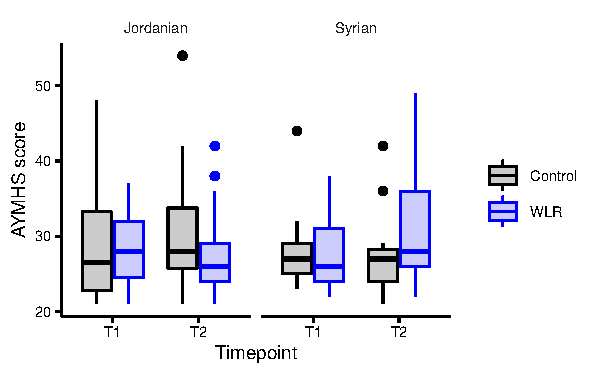
\includegraphics{WLR-analyses-report_files/figure-latex/unnamed-chunk-37-1} 

}

\caption{Distress scores across 2 timepoints}\label{fig:unnamed-chunk-37}
\end{figure}

\begin{longtable}[]{@{}lrrr@{}}
\caption{Distress: ANOVA-Type Statistc (ATS). 2 time points
only.}\tabularnewline
\toprule
& Statistic & df & p-value\tabularnewline
\midrule
\endfirsthead
\toprule
& Statistic & df & p-value\tabularnewline
\midrule
\endhead
wlr\_group & 0.2732606 & 1 & 0.6011528\tabularnewline
nationality & 0.2901686 & 1 & 0.5901125\tabularnewline
time & 3.4912129 & 1 & 0.0616954\tabularnewline
wlr\_group:nationality & 0.0003559 & 1 & 0.9849496\tabularnewline
wlr\_group:time & 0.0892181 & 1 & 0.7651736\tabularnewline
nationality:time & 0.7210084 & 1 & 0.3958133\tabularnewline
wlr\_group:nationality:time & 6.6378831 & 1 & 0.0099832\tabularnewline
\bottomrule
\end{longtable}

\begin{longtable}[]{@{}lrrrr@{}}
\caption{Distress: Modified ANOVA-Type Statistic for the
between-subjects factors. 2 time points only.}\tabularnewline
\toprule
& Statistic & df1 & df2 & p-value\tabularnewline
\midrule
\endfirsthead
\toprule
& Statistic & df1 & df2 & p-value\tabularnewline
\midrule
\endhead
wlr\_group & 0.2732606 & 1 & 43.12443 & 0.6038283\tabularnewline
nationality & 0.2901686 & 1 & 43.12443 & 0.5928825\tabularnewline
wlr\_group:nationality & 0.0003559 & 1 & 43.12443 &
0.9850366\tabularnewline
\bottomrule
\end{longtable}

\newpage

\hypertarget{arab-youth-mental-health-scale-aymhs-1}{%
\subsubsection{Arab Youth Mental Health Scale
(AYMHS)}\label{arab-youth-mental-health-scale-aymhs-1}}

\begin{figure}[H]

{\centering \includegraphics{WLR-analyses-report_files/figure-latex/unnamed-chunk-40-1} 

}

\caption{Mental health (AYMHS) scores across timepoints}\label{fig:unnamed-chunk-40}
\end{figure}

\begin{longtable}[]{@{}lrrr@{}}
\caption{Mental health (AYMHS): ANOVA-Type Statistc (ATS). 2 time points
only.}\tabularnewline
\toprule
& Statistic & df & p-value\tabularnewline
\midrule
\endfirsthead
\toprule
& Statistic & df & p-value\tabularnewline
\midrule
\endhead
wlr\_group & 0.0008576 & 1 & 0.9766380\tabularnewline
nationality & 0.0024131 & 1 & 0.9608208\tabularnewline
time & 2.2759074 & 1 & 0.1313982\tabularnewline
wlr\_group:nationality & 0.6510359 & 1 & 0.4197426\tabularnewline
wlr\_group:time & 0.1778623 & 1 & 0.6732168\tabularnewline
nationality:time & 0.0320515 & 1 & 0.8579147\tabularnewline
wlr\_group:nationality:time & 7.4279115 & 1 & 0.0064220\tabularnewline
\bottomrule
\end{longtable}

\begin{longtable}[]{@{}lrrrr@{}}
\caption{Mental health (AYMHS): Modified ANOVA-Type Statistic for the
between-subjects factors. 2 time points only.}\tabularnewline
\toprule
& Statistic & df1 & df2 & p-value\tabularnewline
\midrule
\endfirsthead
\toprule
& Statistic & df1 & df2 & p-value\tabularnewline
\midrule
\endhead
wlr\_group & 0.0008576 & 1 & 49.63691 & 0.9767554\tabularnewline
nationality & 0.0024131 & 1 & 49.63691 & 0.9610179\tabularnewline
wlr\_group:nationality & 0.6510359 & 1 & 49.63691 &
0.4235920\tabularnewline
\bottomrule
\end{longtable}

\newpage

\hypertarget{post-hoc-tests}{%
\subsubsection{Post-hoc tests}\label{post-hoc-tests}}

Some of the analyses revealed significant changes in the scores that
could be attributed to the WLR reading program. Here I use the same non
parametric approach to do post-hoc comparisons. There are three tables,
one for optimism, one for distress and one for mental health. Control of
family-wise error rate is done by applying the Bonferroni correction:
the adjusted p-value is the p-value multiplied by the number of
comparisons, 4, correspondign to alpha level of 0.0125.\footnote{A more
  restrictive control perhaps would be to consider this a family of 3
  times 4 = 12 comparisons, corresponding to an alpha level of 0.00416,
  in which case the only remaining significant comparison would be
  Syrian, WLR: T2 vs T1, with a p-value of =0.0155.}

\begin{longtable}[]{@{}rrrrl@{}}
\caption{Post-hoc comparisons for Optimism scale. The table also show
the adjusted p value (Bonferroni corrected).}\tabularnewline
\toprule
Statistic & df & p-value & p\_adjusted & Comparison\tabularnewline
\midrule
\endfirsthead
\toprule
Statistic & df & p-value & p\_adjusted & Comparison\tabularnewline
\midrule
\endhead
5.9273992 & 1 & 0.0149072 & 0.0596289 & Syrian, WLR: T2 vs
T1\tabularnewline
0.1564633 & 1 & 0.6924338 & 1.0000000 & Syrian, control: T2 vs
T1\tabularnewline
0.3577598 & 1 & 0.5497531 & 1.0000000 & Jordanian, WLR: T2 vs
T1\tabularnewline
7.8400000 & 1 & 0.0051103 & 0.0204410 & Jordanian, control: T2 vs
T1\tabularnewline
\bottomrule
\end{longtable}

\begin{longtable}[]{@{}rrrrl@{}}
\caption{Post-hoc comparisons for distress scale (HDS). The table also
show the adjusted p value (Bonferroni corrected).}\tabularnewline
\toprule
Statistic & df & p-value & p\_adjusted & Comparison\tabularnewline
\midrule
\endfirsthead
\toprule
Statistic & df & p-value & p\_adjusted & Comparison\tabularnewline
\midrule
\endhead
7.1439114 & 1 & 0.0075219 & 0.0300876 & Syrian, WLR: T2 vs
T1\tabularnewline
0.0000000 & 1 & NA & NA & Syrian, control: T2 vs T1\tabularnewline
0.5597584 & 1 & 0.4543576 & 1.0000000 & Jordanian, WLR: T2 vs
T1\tabularnewline
2.6041406 & 1 & 0.1065849 & 0.4263397 & Jordanian, control: T2 vs
T1\tabularnewline
\bottomrule
\end{longtable}

\begin{longtable}[]{@{}rrrrl@{}}
\caption{Post-hoc comparisons for meantal health scale (AYMHS). The
table also show the adjusted p value (Bonferroni
corrected).}\tabularnewline
\toprule
Statistic & df & p-value & p\_adjusted & Comparison\tabularnewline
\midrule
\endfirsthead
\toprule
Statistic & df & p-value & p\_adjusted & Comparison\tabularnewline
\midrule
\endhead
10.3541699 & 1 & 0.0012918 & 0.0051673 & Syrian, WLR: T2 vs
T1\tabularnewline
0.5678776 & 1 & 0.4511035 & 1.0000000 & Syrian, control: T2 vs
T1\tabularnewline
0.2471749 & 1 & 0.6190714 & 1.0000000 & Jordanian, WLR: T2 vs
T1\tabularnewline
2.1470646 & 1 & 0.1428428 & 0.5713710 & Jordanian, control: T2 vs
T1\tabularnewline
\bottomrule
\end{longtable}

\newpage

Same tests as in previous page, but using Wilcoxon signed rank test.

\begin{longtable}[]{@{}rrrlr@{}}
\caption{Post-hoc comparisons for Optimism scale (Wilcoxon signed rank
tests). The table also show the adjusted p value (Bonferroni
corrected).}\tabularnewline
\toprule
statistic & p.value & p\_adjusted & Comparison &
p.adjusted.BH\tabularnewline
\midrule
\endfirsthead
\toprule
statistic & p.value & p\_adjusted & Comparison &
p.adjusted.BH\tabularnewline
\midrule
\endhead
66.0 & 0.0360975 & 0.1443899 & Syrian, WLR: T2 vs T1 &
0.0721949\tabularnewline
23.5 & 0.9512007 & 1.0000000 & Syrian, control: T2 vs T1 &
0.9512007\tabularnewline
92.0 & 0.4701008 & 1.0000000 & Jordanian, WLR: T2 vs T1 &
0.6268010\tabularnewline
50.0 & 0.0232606 & 0.0930425 & Jordanian, control: T2 vs T1 &
0.0721949\tabularnewline
\bottomrule
\end{longtable}

\begin{longtable}[]{@{}rrrlr@{}}
\caption{Post-hoc comparisons for distress scale (HDS), Wilcoxon signed
rank tests. The table also show the adjusted p value (Bonferroni
corrected).}\tabularnewline
\toprule
statistic & p.value & p\_adjusted & Comparison &
p.adjusted.BH\tabularnewline
\midrule
\endfirsthead
\toprule
statistic & p.value & p\_adjusted & Comparison &
p.adjusted.BH\tabularnewline
\midrule
\endhead
19.5 & 0.0229575 & 0.0918300 & Syrian, WLR: T2 vs T1 &
0.0918300\tabularnewline
24.0 & 0.7593110 & 1.0000000 & Syrian, control: T2 vs T1 &
0.7593110\tabularnewline
87.0 & 0.6346577 & 1.0000000 & Jordanian, WLR: T2 vs T1 &
0.7593110\tabularnewline
46.5 & 0.0929422 & 0.3717688 & Jordanian, control: T2 vs T1 &
0.1858844\tabularnewline
\bottomrule
\end{longtable}

\begin{longtable}[]{@{}rrrlr@{}}
\caption{Post-hoc comparisons for meantal health scale (AYMHS); Wilcoxon
signed rank tests. The table also show the adjusted p value (Bonferroni
corrected).}\tabularnewline
\toprule
statistic & p.value & p\_adjusted & Comparison &
p.adjusted.BH\tabularnewline
\midrule
\endfirsthead
\toprule
statistic & p.value & p\_adjusted & Comparison &
p.adjusted.BH\tabularnewline
\midrule
\endhead
6.5 & 0.0206066 & 0.0824263 & Syrian, WLR: T2 vs T1 &
0.0824263\tabularnewline
41.5 & 0.4749361 & 1.0000000 & Syrian, control: T2 vs T1 &
0.6332481\tabularnewline
89.0 & 0.8957066 & 1.0000000 & Jordanian, WLR: T2 vs T1 &
0.8957066\tabularnewline
18.5 & 0.0634621 & 0.2538486 & Jordanian, control: T2 vs T1 &
0.1269243\tabularnewline
\bottomrule
\end{longtable}

\newpage

\hypertarget{post-hoc-tests-t3-vs-t1}{%
\subsubsection{Post-hoc tests: T3 vs T1}\label{post-hoc-tests-t3-vs-t1}}

\begin{longtable}[]{@{}rrrrl@{}}
\caption{Post-hoc comparisons for Optimism scale. The table also show
the adjusted p value (Bonferroni corrected).}\tabularnewline
\toprule
Statistic & df & p-value & p\_adjusted & Comparison\tabularnewline
\midrule
\endfirsthead
\toprule
Statistic & df & p-value & p\_adjusted & Comparison\tabularnewline
\midrule
\endhead
1.5519268 & 1 & 0.2128512 & 0.8514048 & Syrian, WLR: T3 vs
T1\tabularnewline
0.0917431 & 1 & 0.7619727 & 1.0000000 & Syrian, control: T3 vs
T1\tabularnewline
0.0054735 & 1 & 0.9410241 & 1.0000000 & Jordanian, WLR: T3 vs
T1\tabularnewline
1.7553047 & 1 & 0.1852112 & 0.7408450 & Jordanian, control: T3 vs
T1\tabularnewline
\bottomrule
\end{longtable}

\begin{longtable}[]{@{}rrrrl@{}}
\caption{Post-hoc comparisons for distress scale (HDS). The table also
show the adjusted p value (Bonferroni corrected).}\tabularnewline
\toprule
Statistic & df & p-value & p\_adjusted & Comparison\tabularnewline
\midrule
\endfirsthead
\toprule
Statistic & df & p-value & p\_adjusted & Comparison\tabularnewline
\midrule
\endhead
7.9950150 & 1 & 0.0046906 & 0.0187625 & Syrian, WLR: T3 vs
T1\tabularnewline
0.0232875 & 1 & 0.8787117 & 1.0000000 & Syrian, control: T3 vs
T1\tabularnewline
2.9827353 & 1 & 0.0841569 & 0.3366278 & Jordanian, WLR: T3 vs
T1\tabularnewline
5.5867902 & 1 & 0.0180964 & 0.0723857 & Jordanian, control: T3 vs
T1\tabularnewline
\bottomrule
\end{longtable}

\begin{longtable}[]{@{}rrrrl@{}}
\caption{Post-hoc comparisons for meantal health scale (AYMHS). The
table also show the adjusted p value (Bonferroni
corrected).}\tabularnewline
\toprule
Statistic & df & p-value & p\_adjusted & Comparison\tabularnewline
\midrule
\endfirsthead
\toprule
Statistic & df & p-value & p\_adjusted & Comparison\tabularnewline
\midrule
\endhead
0.0034843 & 1 & 0.9529297 & 1.0000000 & Syrian, WLR: T3 vs
T1\tabularnewline
1.3281453 & 1 & 0.2491354 & 0.9965418 & Syrian, control: T3 vs
T1\tabularnewline
1.2463214 & 1 & 0.2642562 & 1.0000000 & Jordanian, WLR: T3 vs
T1\tabularnewline
0.2463343 & 1 & 0.6196681 & 1.0000000 & Jordanian, control: T3 vs
T1\tabularnewline
\bottomrule
\end{longtable}

\newpage

Same tests as in previous page, but using Wilcoxon signed rank test.

\begin{longtable}[]{@{}rrrlr@{}}
\caption{Post-hoc comparisons for Optimism scale (Wilcoxon signed rank
tests). The table also show the adjusted p value (Bonferroni
corrected).}\tabularnewline
\toprule
statistic & p.value & p\_adjusted & Comparison &
p.adjusted.BH\tabularnewline
\midrule
\endfirsthead
\toprule
statistic & p.value & p\_adjusted & Comparison &
p.adjusted.BH\tabularnewline
\midrule
\endhead
21.0 & 0.2675839 & 1.0000000 & Syrian, WLR: T3 vs T1 &
0.5351678\tabularnewline
23.0 & 0.5176341 & 1.0000000 & Syrian, control: T3 vs T1 &
0.6901788\tabularnewline
48.5 & 0.8594663 & 1.0000000 & Jordanian, WLR: T3 vs T1 &
0.8594663\tabularnewline
12.5 & 0.2030918 & 0.8123672 & Jordanian, control: T3 vs T1 &
0.5351678\tabularnewline
\bottomrule
\end{longtable}

\begin{longtable}[]{@{}rrrlr@{}}
\caption{Post-hoc comparisons for distress scale (HDS), Wilcoxon signed
rank tests. The table also show the adjusted p value (Bonferroni
corrected).}\tabularnewline
\toprule
statistic & p.value & p\_adjusted & Comparison &
p.adjusted.BH\tabularnewline
\midrule
\endfirsthead
\toprule
statistic & p.value & p\_adjusted & Comparison &
p.adjusted.BH\tabularnewline
\midrule
\endhead
4.5 & 0.0217387 & 0.0869547 & Syrian, WLR: T3 vs T1 &
0.0869547\tabularnewline
22.5 & 1.0000000 & 1.0000000 & Syrian, control: T3 vs T1 &
1.0000000\tabularnewline
82.5 & 0.2093514 & 0.8374058 & Jordanian, WLR: T3 vs T1 &
0.2791353\tabularnewline
3.0 & 0.0738343 & 0.2953373 & Jordanian, control: T3 vs T1 &
0.1476686\tabularnewline
\bottomrule
\end{longtable}

\begin{longtable}[]{@{}rrrlr@{}}
\caption{Post-hoc comparisons for meantal health scale (AYMHS); Wilcoxon
signed rank tests. The table also show the adjusted p value (Bonferroni
corrected).}\tabularnewline
\toprule
statistic & p.value & p\_adjusted & Comparison &
p.adjusted.BH\tabularnewline
\midrule
\endfirsthead
\toprule
statistic & p.value & p\_adjusted & Comparison &
p.adjusted.BH\tabularnewline
\midrule
\endhead
17.5 & 0.5933057 & 1.0000000 & Syrian, WLR: T3 vs T1 &
0.7344021\tabularnewline
26.5 & 0.2608580 & 1.0000000 & Syrian, control: T3 vs T1 &
0.5217161\tabularnewline
63.0 & 0.2322284 & 0.9289136 & Jordanian, WLR: T3 vs T1 &
0.5217161\tabularnewline
11.5 & 0.7344021 & 1.0000000 & Jordanian, control: T3 vs T1 &
0.7344021\tabularnewline
\bottomrule
\end{longtable}

\newpage

\hypertarget{correlations-between-questionnaire-scores-and-bias-in-emotion-task}{%
\subsection{Correlations between questionnaire scores and bias in
emotion
task}\label{correlations-between-questionnaire-scores-and-bias-in-emotion-task}}

The table reports both Kendall and Spearman rank-correlation
coefficients between bias in happy-sad task and questionnaire score at
T1, each with both the original p-value and the p-value adjusted after
controlling for false discovery rate (\emph{Benjamini--Hochberg
procedure}).

\begin{longtable}[]{@{}lrrrrrr@{}}
\caption{Non-parametric correlation coefficients between questionnaire
scores and bias in HS task.}\tabularnewline
\toprule
quest & kendall & kendall\_p & kendall\_p\_adj & spearman & spearman\_p
& spearman\_p\_adj\tabularnewline
\midrule
\endfirsthead
\toprule
quest & kendall & kendall\_p & kendall\_p\_adj & spearman & spearman\_p
& spearman\_p\_adj\tabularnewline
\midrule
\endhead
OPTIMISM\_1 & 0.2032 & 0.0088 & 0.0694 & 0.2789 & 0.0068 &
0.0544\tabularnewline
TEC & -0.0971 & 0.2016 & 0.4033 & -0.1214 & 0.2463 &
0.4126\tabularnewline
AYMHS\_1 & 0.0499 & 0.4975 & 0.4975 & 0.0724 & 0.4976 &
0.4976\tabularnewline
CRIES\_ADJUSTED & -0.1617 & 0.0461 & 0.1228 & -0.2093 & 0.0465 &
0.1240\tabularnewline
CRIES\_INTRUSION & -0.0745 & 0.3432 & 0.4576 & -0.0994 & 0.3513 &
0.4634\tabularnewline
CRIES\_AVOIDANCE & -0.0858 & 0.2737 & 0.4379 & -0.1198 & 0.2579 &
0.4126\tabularnewline
HIDS\_INSECURITY\_1 & -0.0597 & 0.4196 & 0.4795 & -0.0893 & 0.4054 &
0.4634\tabularnewline
HIDS\_DISTRESS\_1 & 0.1758 & 0.0173 & 0.0694 & 0.2401 & 0.0226 &
0.0905\tabularnewline
\bottomrule
\end{longtable}

\begin{longtable}[]{@{}lrrrrrr@{}}
\caption{Non-parametric correlation coefficients between questionnaire
scores and bias in FA task.}\tabularnewline
\toprule
quest & kendall & kendall\_p & kendall\_p\_adj & spearman & spearman\_p
& spearman\_p\_adj\tabularnewline
\midrule
\endfirsthead
\toprule
quest & kendall & kendall\_p & kendall\_p\_adj & spearman & spearman\_p
& spearman\_p\_adj\tabularnewline
\midrule
\endhead
OPTIMISM\_1 & -0.0788 & 0.3096 & 0.8255 & -0.1022 & 0.3296 &
0.8788\tabularnewline
TEC & -0.1108 & 0.1449 & 0.5796 & -0.1572 & 0.1325 &
0.5299\tabularnewline
AYMHS\_1 & -0.0139 & 0.8502 & 0.9012 & -0.0218 & 0.8384 &
0.8951\tabularnewline
CRIES\_ADJUSTED & -0.0402 & 0.6203 & 0.9012 & -0.0522 & 0.6228 &
0.8951\tabularnewline
CRIES\_INTRUSION & 0.0167 & 0.8319 & 0.9012 & 0.0282 & 0.7922 &
0.8951\tabularnewline
CRIES\_AVOIDANCE & 0.0097 & 0.9012 & 0.9012 & 0.0140 & 0.8951 &
0.8951\tabularnewline
HIDS\_INSECURITY\_1 & -0.1134 & 0.1254 & 0.5796 & -0.1643 & 0.1240 &
0.5299\tabularnewline
HIDS\_DISTRESS\_1 & 0.0176 & 0.8119 & 0.9012 & 0.0290 & 0.7864 &
0.8951\tabularnewline
\bottomrule
\end{longtable}

\newpage

\hypertarget{references}{%
\section*{References}\label{references}}
\addcontentsline{toc}{section}{References}

\hypertarget{refs}{}
\leavevmode\hypertarget{ref-Brunner1999}{}%
Brunner, Edgar, Ulrich Munzel, and Madan L Puri. 1999. ``Rank-Score
Tests in Factorial Designs with Repeated Measures.'' \emph{Journal of
Multivariate Analysis} 70 (2): 286--317.
\url{https://doi.org/10.1006/jmva.1999.1821}.

\leavevmode\hypertarget{ref-Brunner2001}{}%
Brunner, Edgar, and Madan L. Puri. 2001. ``Nonparametric methods in
factorial designs.'' \emph{Statistical Papers} 42 (1): 1--52.
\url{https://doi.org/10.1007/s003620000039}.

\end{document}
